\documentclass[a4paper,11pt]{article}
\usepackage[T5]{fontenc}
\usepackage{lmodern,newunicodechar}
% Original mappings: Copyright 2005 Werner Lemberg <wl@gnu.org>.
% Adaptation for newunicodechar: LPPL version 1.3 or newer.
% Unicode to T5 mappings adapted from VNTeX t5enc.dfu (LPPL 1.3+).
\makeatletter
\newunicodechar{«}{\guillemotleft}
\newunicodechar{»}{\guillemotright}
\newunicodechar{À}{\@tabacckludge`A}
\newunicodechar{Á}{\@tabacckludge'A}
\newunicodechar{Â}{\^A}
\newunicodechar{Ã}{\~A}
\newunicodechar{È}{\@tabacckludge`E}
\newunicodechar{É}{\@tabacckludge'E}
\newunicodechar{Ê}{\^E}
\newunicodechar{Ì}{\@tabacckludge`I}
\newunicodechar{Í}{\@tabacckludge'I}
\newunicodechar{Ò}{\@tabacckludge`O}
\newunicodechar{Ó}{\@tabacckludge'O}
\newunicodechar{Ô}{\^O}
\newunicodechar{Õ}{\~O}
\newunicodechar{Ù}{\@tabacckludge`U}
\newunicodechar{Ú}{\@tabacckludge'U}
\newunicodechar{Ý}{\@tabacckludge'Y}
\newunicodechar{à}{\@tabacckludge`a}
\newunicodechar{á}{\@tabacckludge'a}
\newunicodechar{â}{\^a}
\newunicodechar{ã}{\~a}
\newunicodechar{è}{\@tabacckludge`e}
\newunicodechar{é}{\@tabacckludge'e}
\newunicodechar{ê}{\^e}
\newunicodechar{ì}{\@tabacckludge`\i}
\newunicodechar{í}{\@tabacckludge'\i}
\newunicodechar{ò}{\@tabacckludge`o}
\newunicodechar{ó}{\@tabacckludge'o}
\newunicodechar{ô}{\^o}
\newunicodechar{õ}{\~o}
\newunicodechar{ù}{\@tabacckludge`u}
\newunicodechar{ú}{\@tabacckludge'u}
\newunicodechar{ý}{\@tabacckludge'y}
\newunicodechar{Ă}{\u A}
\newunicodechar{ă}{\u a}
\newunicodechar{Đ}{\DJ}
\newunicodechar{đ}{\dj}
\newunicodechar{Ĩ}{\~I}
\newunicodechar{ĩ}{\~\i}
\newunicodechar{ı}{\i}
\newunicodechar{Ũ}{\~U}
\newunicodechar{ũ}{\~u}
\newunicodechar{Ơ}{\OHORN}
\newunicodechar{ơ}{\ohorn}
\newunicodechar{Ư}{\UHORN}
\newunicodechar{ư}{\uhorn}
\newunicodechar{Ạ}{\d A}
\newunicodechar{ạ}{\d a}
\newunicodechar{Ả}{\h A}
\newunicodechar{ả}{\h a}
\newunicodechar{Ấ}{\@tabacckludge'\ACIRCUMFLEX}
\newunicodechar{ấ}{\@tabacckludge'\acircumflex}
\newunicodechar{Ầ}{\@tabacckludge`\ACIRCUMFLEX}
\newunicodechar{ầ}{\@tabacckludge`\acircumflex}
\newunicodechar{Ẩ}{\h\ACIRCUMFLEX}
\newunicodechar{ẩ}{\h\acircumflex}
\newunicodechar{Ẫ}{\~\ACIRCUMFLEX}
\newunicodechar{ẫ}{\~\acircumflex}
\newunicodechar{Ậ}{\d\ACIRCUMFLEX}
\newunicodechar{ậ}{\d\acircumflex}
\newunicodechar{Ắ}{\@tabacckludge'\ABREVE}
\newunicodechar{ắ}{\@tabacckludge'\abreve}
\newunicodechar{Ằ}{\@tabacckludge`\ABREVE}
\newunicodechar{ằ}{\@tabacckludge`\abreve}
\newunicodechar{Ẳ}{\h\ABREVE}
\newunicodechar{ẳ}{\h\abreve}
\newunicodechar{Ẵ}{\~\ABREVE}
\newunicodechar{ẵ}{\~\abreve}
\newunicodechar{Ặ}{\d\ABREVE}
\newunicodechar{ặ}{\d\abreve}
\newunicodechar{Ẹ}{\d E}
\newunicodechar{ẹ}{\d e}
\newunicodechar{Ẻ}{\h E}
\newunicodechar{ẻ}{\h e}
\newunicodechar{Ẽ}{\~ E}
\newunicodechar{ẽ}{\~ e}
\newunicodechar{Ế}{\@tabacckludge'\ECIRCUMFLEX}
\newunicodechar{ế}{\@tabacckludge'\ecircumflex}
\newunicodechar{Ề}{\@tabacckludge`\ECIRCUMFLEX}
\newunicodechar{ề}{\@tabacckludge`\ecircumflex}
\newunicodechar{Ể}{\h\ECIRCUMFLEX}
\newunicodechar{ể}{\h\ecircumflex}
\newunicodechar{Ễ}{\~\ECIRCUMFLEX}
\newunicodechar{ễ}{\~\ecircumflex}
\newunicodechar{Ệ}{\d\ECIRCUMFLEX}
\newunicodechar{ệ}{\d\ecircumflex}
\newunicodechar{Ỉ}{\h I}
\newunicodechar{ỉ}{\h i}
\newunicodechar{Ị}{\d I}
\newunicodechar{ị}{\d i}
\newunicodechar{Ọ}{\d O}
\newunicodechar{ọ}{\d o}
\newunicodechar{Ỏ}{\h O}
\newunicodechar{ỏ}{\h o}
\newunicodechar{Ố}{\@tabacckludge'\OCIRCUMFLEX}
\newunicodechar{ố}{\@tabacckludge'\ocircumflex}
\newunicodechar{Ồ}{\@tabacckludge`\OCIRCUMFLEX}
\newunicodechar{ồ}{\@tabacckludge`\ocircumflex}
\newunicodechar{Ổ}{\h\OCIRCUMFLEX}
\newunicodechar{ổ}{\h\ocircumflex}
\newunicodechar{Ỗ}{\~\OCIRCUMFLEX}
\newunicodechar{ỗ}{\~\ocircumflex}
\newunicodechar{Ộ}{\d\OCIRCUMFLEX}
\newunicodechar{ộ}{\d\ocircumflex}
\newunicodechar{Ớ}{\@tabacckludge'\OHORN}
\newunicodechar{ớ}{\@tabacckludge'\ohorn}
\newunicodechar{Ờ}{\@tabacckludge`\OHORN}
\newunicodechar{ờ}{\@tabacckludge`\ohorn}
\newunicodechar{Ở}{\h\OHORN}
\newunicodechar{ở}{\h\ohorn}
\newunicodechar{Ỡ}{\~\OHORN}
\newunicodechar{ỡ}{\~\ohorn}
\newunicodechar{Ợ}{\d\OHORN}
\newunicodechar{ợ}{\d\ohorn}
\newunicodechar{Ụ}{\d U}
\newunicodechar{ụ}{\d u}
\newunicodechar{Ủ}{\h U}
\newunicodechar{ủ}{\h u}
\newunicodechar{Ứ}{\@tabacckludge'\UHORN}
\newunicodechar{ứ}{\@tabacckludge'\uhorn}
\newunicodechar{Ừ}{\@tabacckludge`\UHORN}
\newunicodechar{ừ}{\@tabacckludge`\uhorn}
\newunicodechar{Ử}{\h\UHORN}
\newunicodechar{ử}{\h\uhorn}
\newunicodechar{Ữ}{\~\UHORN}
\newunicodechar{ữ}{\~\uhorn}
\newunicodechar{Ự}{\d\UHORN}
\newunicodechar{ự}{\d\uhorn}
\newunicodechar{Ỳ}{\@tabacckludge`Y}
\newunicodechar{ỳ}{\@tabacckludge`y}
\newunicodechar{Ỵ}{\d Y}
\newunicodechar{ỵ}{\d y}
\newunicodechar{Ỷ}{\h Y}
\newunicodechar{ỷ}{\h y}
\newunicodechar{Ỹ}{\~Y}
\newunicodechar{ỹ}{\~y}
\newunicodechar{‌}{\textcompwordmark}
\newunicodechar{–}{\textendash}
\newunicodechar{—}{\textemdash}
\newunicodechar{‘}{\textquoteleft}
\newunicodechar{’}{\textquoteright}
\newunicodechar{‚}{\quotesinglbase}
\newunicodechar{“}{\textquotedblleft}
\newunicodechar{”}{\textquotedblright}
\newunicodechar{„}{\quotedblbase}
\newunicodechar{‰}{\textperthousand}
\newunicodechar{‱}{\textpertenthousand}
\newunicodechar{‹}{\guilsinglleft}
\newunicodechar{›}{\guilsinglright}
\newunicodechar{␣}{\textvisiblespace}
\newunicodechar{–}{\textendash}
\newunicodechar{—}{\textemdash}
\newunicodechar{×}{\ensuremath{\times}}
\newunicodechar{“}{\textquotedblleft}
\newunicodechar{”}{\textquotedblright}
\makeatother

\usepackage[left=2cm,right=2cm,top=2cm,bottom=2cm]{geometry}
\usepackage{amsmath,amssymb,graphicx,booktabs,array,float,caption,fvextra,titlesec,tocloft,needspace}
\usepackage[unicode,hidelinks]{hyperref}
\hypersetup{pdftitle={Báo cáo HRI – Bài thực hành 05: TurtleBot 4 Navigation và YOLO},pdfauthor={Đỗ Việt Anh}}
\setlength{\parindent}{0pt}
\setlength{\parskip}{5pt}
\setlength{\emergencystretch}{3em}
\setlength{\tabcolsep}{4pt}
\renewcommand{\arraystretch}{1.13}
\renewcommand{\contentsname}{Mục lục}
\renewcommand{\figurename}{Hình}
\renewcommand{\tablename}{Bảng}
\titleformat{\section}{\large\bfseries}{\thesection}{.7em}{}[\titlerule]
\titlespacing*{\section}{0pt}{16pt}{9pt}
\titleformat{\subsection}{\normalsize\bfseries}{\thesubsection}{.7em}{}
\titlespacing*{\subsection}{0pt}{10pt}{6pt}
\captionsetup{font={small,it},labelfont={bf,up},labelsep=colon,skip=5pt}
\setlength{\cftbeforesecskip}{4pt}
\setlength{\cftbeforesubsecskip}{1pt}
\fvset{fontsize=\footnotesize,breaklines=true,breakanywhere=true,breaksymbolleft={},frame=single,framesep=3pt}
\newcommand{\code}[1]{\nolinkurl{#1}}
\newcommand{\fig}[3]{\begin{figure}[H]\centering\includegraphics[width=#2\linewidth]{#1}\caption{#3}\end{figure}}
\raggedbottom
\begin{document}
\hypersetup{pageanchor=false}
\begin{titlepage}
\thispagestyle{empty}
\centering
\vspace*{1.5cm}
{\large\bfseries ĐẠI HỌC QUỐC GIA HÀ NỘI\\[3pt]TRƯỜNG ĐẠI HỌC CÔNG NGHỆ\par}
\vspace{.5cm}

\includegraphics[width=3.2cm]{uet_logo.png}\par
\vspace{.35cm}
{\LARGE\bfseries BÁO CÁO HRI\par}
{\Large BÀI THỰC HÀNH 05\par}
\vspace{.1cm}
{\Large\bfseries TURTLEBOT 4 LOCALIZATION\\AUTONOMOUS NAVIGATION \& YOLO\par}
\vspace{1.7cm}
\begin{tabular}{@{}ll@{}}
\textbf{Họ và tên sinh viên:}&Đỗ Việt Anh\\[8pt]
\textbf{Mã sinh viên:}&23020719\\[8pt]
\textbf{Lớp:}&K68E-RE\\[8pt]
\textbf{Giảng viên hướng dẫn:}&Kỹ sư Nguyễn Quốc Bảo
\end{tabular}
\vfill
Mã nguồn GitHub: \href{@REPO_URL@}{turtlebot4\_bai05}\\[3pt]
Video demo: @VIDEO_COVER@
\vspace{.25cm}
\end{titlepage}
\pagenumbering{roman}
\hypersetup{pageanchor=true}
\tableofcontents
\clearpage
\pagenumbering{arabic}

\section{Tổng quan công việc tuần 5}

Bài thực hành 05 sử dụng lại bản đồ môi trường maze đã lưu ở tuần 4 để định vị
TurtleBot 4 bằng AMCL, điều khiển robot tự động qua ba điểm mục tiêu bằng code và
nhận diện vật thể từ camera RGB bằng YOLO. Công việc được triển khai theo trình tự:
khởi chạy đúng world; nạp map; cho robot ra khỏi dock và khởi tạo pose; chờ AMCL/Nav2
sẵn sàng; chạy node điều hướng và node nhận diện đồng thời; ghi kết quả để đánh giá.

So với tuần 4 đặt goal bằng RViz, tuần này em đưa danh sách pose vào file cấu hình
và dùng \code{nav2_simple_commander} để gửi lần lượt từng goal. Camera được xử lý ở
node riêng nhằm tách vòng nhận ảnh/suy luận khỏi chương trình gửi action. Bản cập nhật
ngày 20/10/2026 sử dụng số liệu và ảnh camera từ lượt \code{@RUN_ID@}, chạy source
commit \code{@CODE_COMMIT@}. Các lượt cũ, gồm run04, được giữ lại để đối chiếu.

\section{Yêu cầu bài toán và môi trường sử dụng}
\subsection{Yêu cầu cần đáp ứng}

Robot phải nạp được hai file \code{map.yaml}, \code{map.pgm} của tuần trước trong
cùng world maze. Sau khi thiết lập Initial Pose, robot và dữ liệu \code{/scan}
phải tương đối khớp bản đồ trên RViz2. Chương trình gửi ít nhất ba goal thuộc các
khu vực khác nhau trong frame \code{map}, chờ kết quả goal hiện tại rồi mới chuyển
sang goal tiếp theo. Trong lúc chạy không phát teleop và không đặt Nav2 Goal bằng chuột.

Node YOLO subscribe ảnh RGB, chuyển Image message sang OpenCV bằng
\code{cv_bridge}, suy luận mô hình, vẽ bounding box kèm class/confidence và in
thông tin ra terminal. Video cần thể hiện navigation hoạt động cùng cửa sổ nhận diện.

\subsection{Các thành phần phần mềm}
\begin{table}[H]\centering\small
\begin{tabular}{@{}p{2.5cm}p{4.4cm}p{8.8cm}@{}}\toprule
Thành phần & Môi trường sử dụng & Vai trò\\\midrule
Hệ điều hành & Ubuntu 22.04 & Chạy trực tiếp trên máy Linux.\\
ROS 2 & Humble & Node, topic, action, TF và simulation time.\\
Mô phỏng & Ignition Gazebo Fortress & World maze, TurtleBot 4 Standard và sensor.\\
Localization & MapServer + AMCL & Nạp map, ước lượng pose và TF.\\
Navigation & Nav2 + Simple Commander & Navfn global planner, DWB local controller.\\
Nhận diện & Ultralytics, YOLO-World TorchScript & Suy luận ảnh RGB với confidence 0,12; imgsz=960.\\
Xử lý ảnh & OpenCV 4.11.0, cv\_bridge & Chuyển ảnh, annotate và hiển thị.\\
Tính toán & PyTorch 2.11.0+cu130, CUDA & Chạy YOLO trên GPU khi khả dụng.\\
Hiển thị & RViz2, Gazebo GUI, OpenCV & Map, scan, pose, path và detection.\\\bottomrule
\end{tabular}
\caption{Phần mềm được sử dụng trong Bài 05.}
\end{table}

\Needspace{18\baselineskip}
\section{Cấu trúc hệ thống và luồng hoạt động}
\subsection{Cấu trúc thư mục}
Các file chính dùng trong chương trình được bố trí như sau:
\begin{Verbatim}
bai05_turtlebot4/
|-- launch/demo.launch.py
|-- scripts/
|   |-- run_demo.sh
|   |-- arrange_windows.py
|   |-- navigate_goals.py
|   `-- yolo_detector.py
|-- config/
|   |-- goals.yaml
|   |-- localization.yaml
|   |-- nav2.yaml
|   `-- gazebo_gui.config
|-- maps/map.yaml, map.pgm
|-- worlds/maze_yolo.sdf, placements.yaml
|-- models/
|   |-- malevisitoronphone/
|   |-- fire_extinguisher/
|   `-- yolo_world_furniture.torchscript
|-- rviz/navigation.rviz
|-- docs/
`-- package.xml, CMakeLists.txt, README.md, LICENSE, NOTICE
\end{Verbatim}

\textbf{Chạy chương trình.}
\code{scripts/run_demo.sh} nạp môi trường ROS, build package và tạo thư mục lưu
kết quả. Script gọi \code{launch/demo.launch.py} để mở Gazebo, robot, AMCL, Nav2,
RViz và YOLO. \code{scripts/arrange_windows.py} căn ba cửa sổ để dễ quan sát và quay video.

\textbf{Điều hướng robot.}
\code{scripts/navigate_goals.py} đọc danh sách đích, cho robot rời dock rồi gửi
lần lượt ba goal tới Nav2. Chương trình chờ kết quả và kiểm tra va chạm trước
khi chuyển goal. File này cũng lưu kết quả vào \code{goal_results.json}, ghi
quỹ đạo vào \code{trajectory.csv} và hiển thị tên các goal trên RViz.

\textbf{Nhận diện từ camera.}
\code{scripts/yolo_detector.py} nhận ảnh RGB, chuyển sang OpenCV và chạy YOLO.
Khi nhận ra người hoặc bình chữa cháy, node vẽ khung cùng nhãn lên ảnh,
hiển thị kết quả và lưu ảnh gốc/ảnh đã vẽ khung để đối chiếu.

\textbf{Các file trong \code{config/}.}
\code{goals.yaml} lưu tọa độ, hướng dừng và thời gian chờ của ba goal.
\code{localization.yaml} lưu cài đặt AMCL để xác định vị trí robot trên map.
\code{nav2.yaml} chứa các cài đặt tìm đường, tránh vật cản, tốc độ và điều kiện
xác nhận đã tới đích. \code{gazebo_gui.config} lưu góc nhìn/cách hiển thị Gazebo.

\textbf{Bản đồ và môi trường.}
Trong \code{maps/}, \code{map.pgm} là ảnh bản đồ, còn \code{map.yaml} lưu đường dẫn
ảnh, độ phân giải và gốc tọa độ. Cả hai giữ nguyên từ tuần 4.
\code{worlds/maze_yolo.sdf} tạo tường và đặt người, bình trong Gazebo;
\code{placements.yaml} ghi lại vị trí để dễ kiểm tra. Khi đổi vị trí vật thể,
cần sửa pose trong SDF và cập nhật YAML tương ứng.

\textbf{Model và hiển thị.}
\code{models/malevisitoronphone/} và \code{models/fire_extinguisher/} chứa model 3D
của người và bình. \code{yolo_world_furniture.torchscript} là model YOLO dùng để
nhận diện ảnh. \code{rviz/navigation.rviz} lưu các lớp map, LiDAR, đường đi,
marker goal và camera RGB để RViz mở sẵn đúng giao diện.

\textbf{Khai báo package và tài liệu.}
\code{package.xml} khai báo các thư viện ROS cần dùng; \code{CMakeLists.txt}
quy định các file được cài khi build. \code{README.md} hướng dẫn cài đặt và chạy,
\code{LICENSE}/\code{NOTICE} ghi giấy phép và nguồn tài nguyên.
\code{docs/} chứa báo cáo, LaTeX, hình và log run10. Kết quả của lượt chạy mới
được ghi vào thư mục \code{output_dir} đã chọn.

\subsection{Sơ đồ khối các thành phần}
\fig{../results/system_flow.pdf}{1.0}{Luồng dữ liệu Localization, Navigation và YOLO. Hai node bài tập sử dụng chung dữ liệu mô phỏng nhưng chạy ở hai process.}

\subsection{Các node và thành phần chính}
\begin{table}[H]\centering\small
\begin{tabular}{@{}p{5.3cm}p{10.4cm}@{}}\toprule
Thành phần & Chức năng\\\midrule
Gazebo và ROS--Gazebo bridge & Mô phỏng robot/sensor; chuyển scan, ảnh, odometry và clock sang ROS.\\
robot\_state\_publisher & Xuất TF của thân robot và các sensor.\\
map\_server / amcl & Phát occupancy map, cập nhật particle và TF \(map\rightarrow odom\).\\
planner\_server / controller\_server & Lập global path và tính lệnh vận tốc để bám path.\\
bt\_navigator / behavior\_server & Điều phối NavigateToPose và hành vi hỗ trợ.\\
lifecycle\_manager & Configure/activate các node Nav2.\\
bai05\_route\_navigator & Undock, khởi tạo AMCL, gửi goal tuần tự, lưu action result và telemetry.\\
bai05\_yolo\_detector & Nhận Image, cv\_bridge, YOLO, publish ảnh/JSON detection và hiển thị.\\\bottomrule
\end{tabular}
\caption{Chức năng các thành phần chính.}
\end{table}

\subsection{Topic, action và hệ tọa độ}
Các node dùng topic để gửi dữ liệu như ảnh, scan và vị trí. Yêu cầu đi đến đích
hoặc rời dock dùng action để chương trình có thể chờ và nhận kết quả.

\textbf{Bản đồ và vị trí robot.}
\code{map_server} phát bản đồ qua \code{/map}; LiDAR gửi khoảng cách tới vật cản
qua \code{/scan}. AMCL dùng hai nguồn này cùng chuyển động robot để tìm vị trí
trên map, rồi phát \code{/amcl_pose}. \code{/odom} cung cấp chuyển động và vận tốc
để Nav2 điều khiển robot. Node điều hướng lưu vị trí từ AMCL và vận tốc từ
\code{/odom} vào log.

\textbf{Khởi tạo và gửi goal.}
Trong mô phỏng, \code{/sim_ground_truth_pose} cung cấp vị trí robot từ Gazebo;
node dùng nó để đặt vị trí ban đầu cho AMCL qua \code{/initialpose} và đối chiếu log.
Node gửi từng đích qua action \code{/navigate_to_pose}, chờ kết thúc rồi mới gửi
đích tiếp theo. Nếu \code{/dock_status} cho biết robot đang ở dock, chương trình
thực hiện action \code{/undock} trước.

\textbf{Chuyển động và va chạm.}
Nav2 đưa ra lệnh vận tốc qua \code{/cmd_vel}; \code{linear.x} là tốc độ đi thẳng,
\code{angular.z} là tốc độ quay. \code{/hazard_detection} và \code{/bumper_contact}
báo các va chạm để node ghi nhận, kiểm tra cùng kết quả mỗi goal trước khi đi tiếp.

\textbf{Camera và YOLO.}
\code{/oakd/rgb/preview/image_raw} đưa ảnh RGB từ camera tới RViz và node YOLO.
Sau nhận diện, \code{/bai05/yolo/image} chứa ảnh đã vẽ khung;
\code{/bai05/yolo/detections} chứa nhãn, confidence và tọa độ khung dạng JSON.
Tọa độ khung tính theo pixel ảnh, chưa phải vị trí vật thể trên bản đồ.
YOLO chỉ nhận diện; Nav2 tránh vật cản bằng LiDAR và costmap.

\textbf{Thông tin hiển thị.}
Node điều hướng gửi trạng thái đang đi goal nào/đã xong qua
\code{/bai05/mission_status} để YOLO ghi lên ảnh. \code{/waypoints} chứa các nhãn
Goal 1--3 cho RViz; các nhãn này chỉ đánh dấu vị trí, không điều khiển robot.

\textbf{Hệ tọa độ và thời gian.}
\code{/tf}, \code{/tf_static} giúp liên hệ vị trí bản đồ, thân robot và cảm biến:
\[
\texttt{map}\longrightarrow\texttt{odom}\longrightarrow
\texttt{base\_link}\longrightarrow\texttt{sensor}.
\]
\code{map} gắn với bản đồ; \code{odom} theo dõi chuyển động;
\code{base_link} gắn với thân robot, còn các frame sensor gắn với LiDAR/camera.
RViz chọn Fixed Frame = map để đặt các dữ liệu đúng vị trí. Ba goal cũng dùng
frame map, với \(x,y\) là vị trí và yaw là hướng dừng.

\code{/clock} cung cấp thời gian mô phỏng. Các node dùng \code{use_sim_time=true}
để ảnh, pose và TF cùng theo đồng hồ này; riêng timeout và khoảng dừng giữa
các goal dùng thời gian thực. Log giữ timestamp từng nguồn để kiểm tra khi đối chiếu.

\subsection{Luồng hoạt động khi chạy}

Launch mở mô phỏng và nạp map cùng cấu hình Nav2. Node navigation chờ clock,
ground truth và dock status; nếu robot đang dock thì gửi action Undock và chờ thành công.
Pose Gazebo sau undock được dùng làm ước lượng khởi tạo AMCL. Khi AMCL/Nav2 active,
node đọc goals.yaml, gửi Goal 1, chờ action kết thúc, ghi kết quả, dừng
khoảng 6 giây wall time rồi tiếp tục Goal 2 và Goal 3; không gửi pose quan sát chen giữa.
Mỗi goal có timeout 600 giây wall time. Lượt thất bại, timeout hoặc có
BUMP/contact làm nhiệm vụ dừng để kiểm tra. Không có lệnh teleop trong vòng lặp này.

Node YOLO nhận ảnh mới nhất bằng QoS best effort, depth 1. Callback subscriber chỉ
giữ ảnh; timer 0,25 giây mô phỏng thực hiện suy luận. Cách này hạn chế xử lý hàng đợi
ảnh cũ. Node publish ảnh annotate và JSON, lưu log, đồng thời mở cửa sổ OpenCV.
Mission status được truyền qua topic để hiển thị goal đang chạy trên cửa sổ camera.

\section{Môi trường mô phỏng và nhiệm vụ thực hành}
\subsection{Bố trí môi trường}

World maze gồm tường, hành lang, ngã rẽ và các vùng mở như tuần trước. Robot bắt
đầu tại gần tâm world cùng dock sạc. Scene cuối giữ một model MaleVisitorOnPhone
tại $(-3;5)$, một bình chữa cháy gần Goal 1 tại $(-7,8;6,2)$ và một bình trên tuyến
Goal 2 đến Goal 3 tại $(-1,8;-5,5)$. Em bỏ bàn, ghế và người ở vị trí chạm/xuyên tường.
Hai bình là model hình học SDF có collision, người là model Gazebo Fuel.
Node nhận diện nhận ảnh RGB thật từ camera mô phỏng.

\fig{../results/scene_layout.pdf}{.67}{Sơ đồ bố trí scene cuối trên map tuần 4, lấy từ world SDF của run10. Ký hiệu người/bình là vị trí model trong mô phỏng; các vật thêm vào không sửa file map.}

Vị trí vật thể phụ thuộc bố trí tường nên không phải lúc nào camera cũng nhìn thấy.
Tại một số hướng, tường che phần lớn khung hình. Khi đánh giá YOLO cần đối chiếu
ảnh RGB thực tế thay vì giả định model đã thêm luôn xuất hiện trong ảnh.

\subsection{Nhiệm vụ}

Nhiệm vụ gồm ba phần: định vị trên bản đồ đã có; tự động đi qua ba goal bằng node
Python; nhận diện bằng YOLO trong lúc di chuyển hoặc dừng tại goal. Các goal được
khảo sát theo vùng trống của map và lưu cố định trong cấu hình để tái hiện lượt chạy.

\section{Xây dựng bản đồ bằng SLAM Toolbox}
\subsection{Nguyên lý và thao tác mapping}

Ở tuần 4, SLAM Toolbox kết hợp scan LiDAR với odometry/TF để ước lượng pose và
xây occupancy grid 2D khi robot được điều khiển khảo sát. Trong bài tuần 5, em dùng
lại hai file map đã lưu, không chạy lại SLAM để tạo map mới. Mục này giữ vị trí trong
cấu trúc báo cáo để trình bày nguồn map và mối liên hệ với bài trước.

\subsection{Bản đồ đã lưu}
\fig{../results/map_original.png}{.58}{Bản đồ PGM tuần 4 được nạp lại nguyên byte trong bài tuần 5.}
\begin{table}[H]\centering\small
\begin{tabular}{@{}ll@{}}\toprule
Thuộc tính & Giá trị\\\midrule
Kích thước & 401 $\times$ 401 ô\\
Resolution & 0,05 m/ô\\
Origin & $(-10;-10;0)$\\
Mode / negate & trinary / 0\\
Occupied / free threshold & 0,65 / 0,25\\\bottomrule
\end{tabular}
\caption{Thông số map từ YAML và PGM.}
\end{table}

Hai file được sao chép từ repository \url{https://github.com/vanhhhhh512/turtlebot4_bai04}
và đối chiếu SHA256 với bản cài từ clone GitHub. Bản đồ thể hiện tường
và các cấu trúc đã quét; các model mới của tuần 5 không được ghi vào map tĩnh.
Thông tin vật cản mới phụ thuộc sensor và costmap trong thời gian chạy.

\section{Localization sau khi nạp lại bản đồ}
\subsection{Trình tự khởi tạo}

MapServer đọc map.yaml và phát \code{/map}. AMCL sử dụng bản đồ, scan và chuyển
động odometry để cập nhật pose cùng transform \(map\rightarrow odom\).
Trong lượt chính, action Undock trả thành công trước khi khởi tạo AMCL.
Initial Pose được lấy từ Gazebo tại \(@INITIAL_POSE@\).

Đây là cách khởi tạo thuận tiện cho mô phỏng, sử dụng ground truth làm đầu vào.
Việc pose ban đầu trùng GT không phải phép đánh giá độc lập độ chính xác AMCL.
Sau khởi tạo, chương trình vẫn chờ AMCL/Nav2 active và đối chiếu scan với map trên RViz.

\subsection{Quan sát localization và đối chiếu log}
\fig{../results/localization_difference.pdf}{1.0}{Chênh lệch XY giữa pose AMCL và Gazebo được lưu trong cùng mẫu telemetry của run10. Hai pose có thể khác timestamp.}

RViz dùng Fixed Frame = map và hiển thị scan cùng tường để kiểm tra localization.
Trong log run10, chênh lệch XY lớn nhất giữa các pose đã lưu là @AMCL_GT_MAX@ m;
không có relocalization giữa tuyến. Giá trị này phản ánh hai snapshot có thể khác
timestamp, không phải phép đo độc lập sai số AMCL đã đồng bộ thời gian. Trạng thái
active chỉ phản ánh node đã kích hoạt; còn cần quan sát scan/map và diễn biến pose.

\section{Navigation với Nav2}
\subsection{Lập kế hoạch và điều khiển}

Node \code{bai05_route_navigator} kế thừa BasicNavigator. Hàm \code{goToPose()}
gửi NavigateToPose trong frame map; \code{isTaskComplete()} cho phép chờ kết quả
trong khi callback telemetry vẫn được xử lý. bt\_navigator điều phối yêu cầu;
planner\_server dùng NavfnPlanner để tạo global path; controller\_server dùng
DWBLocalPlanner cùng local costmap để tính vận tốc. Lệnh được chuyển qua
velocity smoother và \code{/cmd_vel} tới robot.

Cấu hình lưu trong config/nav2.yaml giữ tốc độ thẳng tối đa 0,26 m/s và góc tối đa
1,0 rad/s của controller. Costmap kết hợp bản đồ tĩnh, dữ liệu quan sát và inflation.
Trong bài này YOLO chỉ nhận diện và hiển thị; detection RGB chưa được dùng làm input
tránh vật cản hay thay đổi goal. Tránh va chạm do Nav2/costmap và sensor của robot đảm nhiệm.
Mỗi chặng chỉ có một đích NavigateToPose. Sau Goal 2, chương trình gửi trực tiếp
Goal 3; Nav2 có thể cập nhật đường đi khi costmap thay đổi nhưng đích vẫn là Goal 3.
Việc YOLO nhìn thấy bình không kích hoạt gửi goal hoặc nối thêm đường đi.

\subsection{Ảnh RViz}
\fig{../results/rviz_rgb_camera.png}{1.0}{RViz hiển thị camera OAK-D RGB ở góc trên trái cùng map, scan LiDAR, costmap và path. Ảnh chụp từ lượt \code{corners_run04} minh họa giao diện có RGB trong RViz; số liệu kết quả cập nhật lấy từ run10 ở mục 9.}

Panel \code{OAK-D RGB} dùng display Image, nhận topic \code{/oakd/rgb/preview/image_raw}; camera RGB được hiển thị trực tiếp trong RViz cùng dữ liệu LiDAR/map.

Các dải màu quanh tường thể hiện chi phí vật cản và inflation. Marker Goal 1--3
chỉ hiển thị vị trí trong file cấu hình; marker không phát action hoặc lệnh vận tốc.

\subsection{Thực hiện và phân loại goal}
\begin{table}[H]\centering\small
\begin{tabular}{@{}lrrrl@{}}\toprule
Goal & x (m) & y (m) & yaw (rad) & Hệ tọa độ\\\midrule
@GOAL_TARGET_ROWS@
\bottomrule
\end{tabular}
\caption{Các mục tiêu lưu trong goals.yaml.}
\end{table}

Tọa độ được chọn theo map đã quét và đối chiếu với các khu vực của world.
File cấu hình lưu cả yaw; Publish Point chỉ cho vị trí, hướng kết thúc phải được chọn
riêng. Chương trình lần lượt gọi goToPose, chờ kết quả, kiểm tra SUCCEEDED và
các tín hiệu va chạm rồi mới gửi goal kế tiếp. Không có thao tác Nav2 Goal bằng chuột
hoặc teleop trong lượt run10. Log ghi Goal 2 thành công tại 200,760 giây mô phỏng
và gửi Goal 3 tại 206,115 giây; giữa hai event chỉ có thời gian dừng, không có goal phụ.

\begin{Verbatim}
for goal in goals:
    pose = make_pose(frame_id='map', x=goal.x, y=goal.y, yaw=goal.yaw)
    navigator.goToPose(pose)
    while not navigator.isTaskComplete():
        check_timeout()
    result = navigator.getResult()
    save_result_and_telemetry(result)
    if result != TaskResult.SUCCEEDED or collision_detected:
        stop_mission()
\end{Verbatim}
Đoạn trên tóm tắt thuật toán; mã nguồn thật còn có bước undock, initial pose,
ghi log, kiểm tra timeout và thời gian dừng giữa các goal.

\subsection{Nhận diện vật thể từ camera bằng YOLO}

Node \code{bai05_yolo_detector} subscribe
\code{/oakd/rgb/preview/image_raw} dưới dạng \code{sensor_msgs/msg/Image}, gọi
\code{imgmsg_to_cv2()} với \code{desired_encoding='bgr8'} rồi đưa ảnh vào YOLO-World
TorchScript đi kèm source. Mô hình nhận tham số imgsz=960, confidence=0,12 và device GPU. Ảnh camera thực
trong lượt chạy có kích thước 320$\times$240; imgsz là cấu hình xử lý của model,
không có nghĩa camera cung cấp ảnh 960 pixel gốc. Prompt hình trụ đỏ có dải trắng
được ánh xạ thành nhãn \code{fire extinguisher}; node vẽ/lưu class này cùng \code{person}.

Từ kết quả suy luận, node lấy class, confidence và box xyxy; vẽ nhãn trong khung
ảnh để tránh bị che khi box chạm mép trên. Node publish ảnh \code{bgr8} và JSON
detection có timestamp/frame\_id, đồng thời in thông tin ra terminal. Raw frame và
ảnh annotate được lưu theo định kỳ khi có detection để đối chiếu kết quả.

\begin{figure}[H]\centering
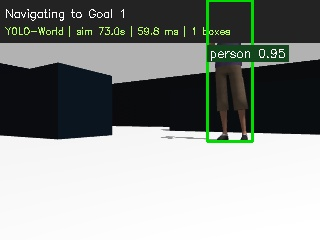
\includegraphics[width=.48\linewidth]{../results/best_person_yolo.jpg}\hfill
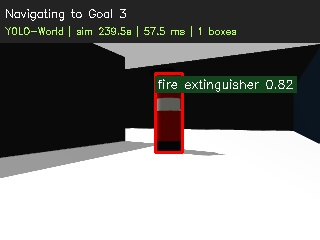
\includegraphics[width=.48\linewidth]{../results/extinguisher_goal3_yolo.jpg}
\caption{Ảnh camera run10 có bbox person (trái, confidence @BEST_PERSON@) và bình trên tuyến Goal 3 (phải, confidence @GOAL3_CONFIDENCE@). Nhãn là dự đoán của model, không phải ground truth.}
\end{figure}

\section{Khó khăn gặp phải và cách xử lý}
\subsection{Bridge sử dụng sai tên world}

Lượt chạy đầu dùng đường dẫn file SDF làm biến world của launch upstream.
Các bridge vì vậy tạo topic có đoạn \code{/world//home/...}, khiến ROS báo lỗi remap.
Em tách đường dẫn file world khỏi tên thực thể world: Gazebo mở file được sinh khi
launch, còn các bridge dùng đúng tên \code{maze}. Lỗi được giữ lại trong log scout.

\subsection{Tham số ROS và đường dẫn plugin mô phỏng}

Tham số device truyền bằng chuỗi số 0 bị launch diễn giải thành integer trong khi
node khai báo string. Cách sửa là dùng ParameterValue với value\_type=str. Tên
weights đổi thành yolo\_model để không trùng model của TurtleBot. Khi chạy Ignition
riêng, cần thêm \code{/opt/ros/humble/lib} vào system plugin path; nếu thiếu,
\code{libign_ros2_control-system.so} không nạp và controller\_manager không xuất hiện.

\subsection{Mô phỏng chậm trên màn hình ảo}

Màn hình desktop đang khóa nên em dùng Xvfb để bố trí/quay các cửa sổ. Lượt chạy
server trên display ảo dùng software rendering và undock bị timeout: log chỉ tiến
được khoảng 3,84 giây simulation khi hết thời gian chờ. Em chuyển server cảm biến
sang display có GPU, còn GUI/RViz/OpenCV vẫn nằm trên display ảo. Sau thay đổi,
robot thực hiện được trọn tuyến. Các lượt lỗi không được tính là demo hoàn thành.

\subsection{Giới hạn quan sát và nhận diện}

Camera đặt thấp nên khi robot gần người, phần đầu có thể nằm ngoài khung ảnh.
Tường làm che khuất model ở một số hướng; YOLO cũng có thể nhầm mặt tường/biên
vật thể thành class khác. Em giữ các detection này trong log để nhận xét thay vì
lọc bỏ khỏi số liệu tổng hợp. Bài hiện chưa có bộ ảnh gán nhãn để tính precision,
recall hoặc mAP, và chưa dùng depth để đo khoảng cách vật thể.
Một phiên bản trước có pose quan sát chen giữa Goal 2 và Goal 3, làm đường hiển thị
đi tới pose phụ thay vì tới Goal 3. Em bỏ bước đó và chuyển bình lên tuyến đi thực tế;
run10 kiểm tra lại toàn bộ ba goal với Nav2 tự xử lý vật cản.

\section{Kết quả đạt được}
\subsection{Mô phỏng, sensor và map}
\begin{table}[H]\centering\small
\begin{tabular}{@{}p{3.2cm}p{12.5cm}@{}}\toprule
Hạng mục & Kết quả\\\midrule
Map & 401$\times$401 ô; 0,05 m/ô; origin $(-10;-10;0)$; SHA256 khớp nguồn tuần 4.\\
Localization & AMCL active; Fixed Frame map và scan hiển thị cùng tường trên RViz.\\
Navigation & @SUCCESS_COUNT@/3 action SUCCEEDED; không có BUMP hazard trong cửa sổ chạy route.\\
Camera RGB & 320$\times$240; subscribe bằng Image và chuyển BGR qua cv\_bridge.\\
Object detection & YOLO-World chạy đồng thời; có ảnh/JSON/log person và fire extinguisher.\\\bottomrule
\end{tabular}
\caption{Kết quả chính của lượt chạy tuần 5.}
\end{table}

\subsection{Kết quả từng navigation goal}
\begin{table}[H]\centering\small
\begin{tabular}{@{}llrrrr@{}}\toprule
Goal & Action & AMCL (m) & $T_{sim}$ (s) & $T_{wall}$ (s) & $e_{goal}$ (m)\\\midrule
@GOAL_ROWS@
\bottomrule\end{tabular}
\caption{Kết quả ba goal theo thứ tự chương trình gửi.}
\end{table}

Tổng quãng đường AMCL của ba lượt là @TOTAL_PATH@ m. Quãng đường được tính
trên chuỗi pose AMCL lấy mẫu mỗi 0,2 giây mô phỏng; mẫu không đổi không làm tăng tổng:
\[
L=\sum_{i=1}^{n}\sqrt{(x_i-x_{i-1})^2+(y_i-y_{i-1})^2},\qquad
e_{goal}=\sqrt{(x_f-x_g)^2+(y_f-y_g)^2}.
\]
Thời gian trong bảng đo từ trước goToPose đến sau khi nhận result và spin thêm
0,5 giây wall để lấy snapshot. Vì vậy nó gồm khoảng chờ phản hồi và ổn định ngắn,
không chỉ là thời gian robot chuyển động. $T_{sim}$ và $T_{wall}$ được giữ riêng.

Sai lệch $e_{goal}$ là khoảng cách từ mẫu AMCL cuối tới tọa độ đích, không phải sai
số localization so với vị trí thật. AMCL và GT cuối có độ lệch timestamp
@STAMP_GAP@ s; snapshot AMCL có thể sớm hơn thời điểm goal checker xác nhận.
SUCCEEDED phản ánh điều kiện goal checker của Nav2. Không suy ra độ chính xác
toàn hệ hoặc sai số yaw từ một mẫu pose cũ.

Các lượt có @HAZARD_MESSAGES@ message hazard được xử lý đến cuối Goal 3 và không
có detection loại BUMP. Không ghi nhận message contact có dữ liệu.
Topic bumper chỉ phát khi có contact; số message bằng 0 cần được đọc cùng
video và log hazard, không phải phép chứng minh độc lập mọi loại va chạm.
Log \code{MISSION_COMPLETE} ghi 3 goal, 0 contact và 0 bump.

\subsection{Quãng đường, thời gian và sai lệch}
\fig{../results/goal_metrics.pdf}{1.0}{Quãng đường AMCL, thời gian mô phỏng và khoảng cách pose cuối--goal từ dữ liệu của ba goal.}
@NAV_OBSERVATION@

\subsection{Quỹ đạo AMCL theo từng goal}
\fig{../results/route_map.pdf}{.72}{Map và toàn bộ quỹ đạo AMCL tuần 5; dấu nhân là goal, vòng tròn là điểm đầu từng đoạn.}
\fig{../results/trajectories.pdf}{1.0}{Quỹ đạo AMCL tách theo goal; vòng tròn là điểm đầu, vuông là điểm cuối, dấu nhân là tọa độ đích.}
Các đường thể hiện pose AMCL đã ghi nhận, không phải global path do planner xuất.
Đoạn đi vòng hoặc các góc rẽ phản ánh bố trí hành lang của maze và lựa chọn của controller.
\fig{../results/obstacle_avoidance.pdf}{.80}{Quỹ đạo Gazebo khi đi Goal 3 quanh bình tại $(-1,8;-5,5)$. Khoảng cách nhỏ nhất giữa tâm robot và tâm bình là @OBSTACLE_DISTANCE@ m; đây không phải khoảng hở giữa hai bề mặt.}

\subsection{Quãng đường tích lũy theo thời gian}
\fig{../results/cumulative_distance.pdf}{1.0}{Tổng độ dời XY liên tiếp của AMCL theo thời gian mô phỏng trong từng goal.}
Đoạn gần ngang cho thấy vị trí AMCL ít thay đổi; chỉ từ biểu đồ không phân biệt
được robot đang quay tại chỗ, đứng chờ hoặc AMCL chưa phát pose mới. Không cộng
quãng đường giữa các goal vào một đoạn đo nếu mẫu thuộc thời gian dừng giữa hai goal.

\subsection{Kết quả nhận diện và đánh giá}
\begin{table}[H]\centering\small
\begin{tabular}{@{}lr@{}}\toprule
Chỉ số & Kết quả\\\midrule
Frame ảnh đã xử lý & @YOLO_FRAMES@\\
Frame có ít nhất một box & @POSITIVE_FRAMES@\\
Box person trên các frame & @PERSON_BOXES@\\
Box fire extinguisher trên các frame & @EXTINGUISHER_BOXES@\\
cv\_bridge + predict, median & @LATENCY_MEDIAN@ ms\\
cv\_bridge + predict, p95 & @LATENCY_P95@ ms\\\bottomrule
\end{tabular}
\caption{Thống kê YOLO trong cửa sổ ghi log của lượt chính.}
\end{table}

@DETECTION_OBSERVATION@
Số box cộng qua các frame không phải số người duy nhất: cùng một người có thể
được phát hiện nhiều lần. Các chỉ số thời gian chỉ tính chuyển ảnh và predict,
chưa tính annotate, publish, vẽ cửa sổ hoặc lưu JPEG; không chuyển trực tiếp
nghịch đảo giá trị này thành FPS end-to-end. Chưa có nhãn ground truth cho toàn
bộ ảnh nên báo cáo không đưa accuracy hoặc mAP.

\section{Cách chạy code}
\subsection{Chạy all bằng một lệnh}

Sau khi cài dependency và build theo README, chạy:
\begin{Verbatim}
cd ~/turtlebot5_github_ws/src/bai05_turtlebot4
./scripts/run_demo.sh
\end{Verbatim}

\begin{table}[H]\centering\small
\begin{tabular}{@{}cp{7.0cm}p{8.1cm}@{}}\toprule
Bước & Thao tác & Kết quả mong đợi\\\midrule
1 & Chạy script run\_demo.sh. & Build các package cần thiết; mở Gazebo, RViz và YOLO.\\
2 & Chờ bootstrap, quan sát pose/scan. & Robot undock; Initial Pose được đặt; Nav2 active.\\
3 & Quan sát chương trình tự chạy route. & Goal1, Goal2, Goal3 được gửi tuần tự bằng code.\\
4 & Quan sát cửa sổ camera và terminal. & Box/class/confidence, JSON và log nhận diện.\\
5 & Chờ MISSION\_COMPLETE, xem output\_dir. & Có kết quả goal, CSV trajectory và ảnh detection.\\
6 & Ctrl+C terminal launch. & Dừng mô phỏng và các node của phiên.\\\bottomrule
\end{tabular}
\caption{Trình tự thao tác tái hiện chương trình.}
\end{table}

Có thể chọn \code{device:=cpu} hoặc truyền weights bằng \code{yolo_model:=...}.
Lượt run10 dùng desktop DISPLAY=:0; script căn ba cửa sổ và tự chọn ROS domain,
Ignition partition riêng cho mỗi phiên. Mặc định dữ liệu lưu ở \code{~/bai05_runs/};
có thể đặt \code{BAI05_OUTPUT_DIR} để chọn thư mục mới cho một lượt.

Source public: \url{@REPO_URL@}.
Source map/localization tuần 4: \url{https://github.com/vanhhhhh512/turtlebot4_bai04}.

Video demo: @VIDEO_BODY@.
Bản code kiểm chứng: commit \code{@CODE_COMMIT@}; số liệu chính: \code{@RUN_ID@}.
Báo cáo và biểu đồ được tái tạo bằng script đi kèm hồ sơ; README repository
chứa lệnh cài đặt/build và cách chạy riêng từng node.

\section{Kiến thức và kỹ năng đã học được}
\subsection{Phân biệt mapping, localization và navigation}

Mapping tạo bản đồ từ sensor và chuyển động; localization ước lượng pose trên map
đã có; navigation dùng pose và costmap để tìm đường rồi điều khiển robot tới goal.
Ở tuần này em dùng map tuần trước cho AMCL và tập trung lập trình phần gửi goal.
Việc có model YOLO nhận diện được người không tự bổ sung người đó vào costmap.

\subsection{Làm việc với hệ tọa độ và thời gian ROS 2}

Pose mục tiêu cần đúng frame và quaternion. Clock mô phỏng khác thời gian thực,
nên đo riêng hai loại thời gian và lưu timestamp của từng nguồn. Khi gặp lỗi TF,
cần kiểm tra node phát transform, thời điểm dữ liệu và trình tự khởi động; trạng thái
hiển thị RViz chỉ là một phần của quá trình kiểm tra.

\subsection{Nhận biết giới hạn của sensor}

LiDAR 2D quan sát mặt phẳng quét, còn RGB phụ thuộc góc nhìn và vật thể có nằm
trong ảnh hay không. Camera thấp có thể chỉ nhìn thấy một phần người; tường hoặc
vật cản che khuất làm detector bỏ sót. Confidence là đầu ra mô hình cho từng box,
không phải bằng chứng chắc chắn class đúng và không phải xác suất hệ thống an toàn.

\subsection{Lập trình node và đánh giá kết quả}

Em nắm được cách dùng action để chờ một nhiệm vụ dài, chuyển trạng thái tuần tự
và dừng khi có lỗi; dùng subscriber/timer để tách nhận ảnh và suy luận; chuyển
Image message sang OpenCV bằng cv\_bridge. Qua log và biểu đồ, em cũng thấy cần
giải thích rõ nguồn dữ liệu, cách tính và trường hợp chưa đo được trước khi kết luận.

\section*{Tài liệu tham khảo}
\addcontentsline{toc}{section}{Tài liệu tham khảo}
\begin{enumerate}
\item TurtleBot 4 User Manual -- Navigator và Simulation.\\
\url{https://turtlebot.github.io/turtlebot4-user-manual/tutorials/turtlebot4_navigator.html}
\item Nav2 Simple Commander API.\\\url{https://docs.nav2.org/commander_api/index.html}
\item Ultralytics -- Model Prediction.\\\url{https://docs.ultralytics.com/modes/predict/}
\item vision\_opencv / cv\_bridge.\\\url{https://github.com/ros-perception/vision_opencv/tree/humble/cv_bridge}
\item Gazebo Fuel -- MaleVisitorOnPhone v2, tác giả Wan Yi Seow, CC BY 4.0. Metadata được giữ trong repository; bình chữa cháy được dựng bằng SDF trong source bài tập.
\end{enumerate}
\end{document}
